\documentclass[./main]{subfiles}

\begin{document}

This part of the thesis deals with tools for and research into Scratch, a visual programming language targeted at young users.

There are two main tools that we created for Scratch: a testing framework Itch and a debugger Blink.

Itch was created in collaboration with FTRPRF, uitelg.

\Vref{ch:blink}, about Blink, is based on a previously published paper:

\begin{itemize}
    \item \fullcite{strijbolBlinkEducationalSoftware2024}
\end{itemize}

The next section of this introduction will introduce Scratch itself: a basic knowledge about how Scratch is used and works is useful for all next chapters.
Afterwards, a list of software artefacts is given.

\chapter{Scratch: the programming language}\label{ch:scratch-the-programming-language}

Scratch is a visual programming language and environment~\autocite{resnickScratchProgrammingAll2009}.
It is block-based, meaning code is represented by blocks with different shapes.
Developed by the Lifelong Kindergarten research group at the MIT Media Lab, beginning in 2002.
Scratch became publicly available in 2007, and has been developed by the Scratch Foundation since 2009.
Its target audience is ages 8 to 16, although it is most commonly used for ages 10 to 14.

It is a widely used programming language: the 2022 annual report of the Scratch Foundation~\autocite{GrowingGlobalCreative2022} states that there are over 50 million users in the online Scratch community, with 120 new projects (the programs) being made.

Blocks can be dragged from the toolbox on the left side of the integrated development environment (\vref{fig:scratch-ide-intro}) to the workspace in the middle and can be stacked together to form scripts.
Each executable script has a hat block that defines when the script should start executing.
Scripts can be started as a result of a user action or when a certain criterium is met during the execution of a program, for example, when a clone is started or a message is broadcast.
Each script is connected to a sprite.
Sprites are objects that are drawn on the screen.
The bottom right corner of the environment contains an editor for sprites and the background, which is a special sprite called Stage that is present in every Scratch project.
All scripts corresponding to the selected sprite are shown in the workspace (middle).
The canvas in the top right corner of the environment shows the execution of the project.

\begin{figure}
    \centering
    \begin{wide}
        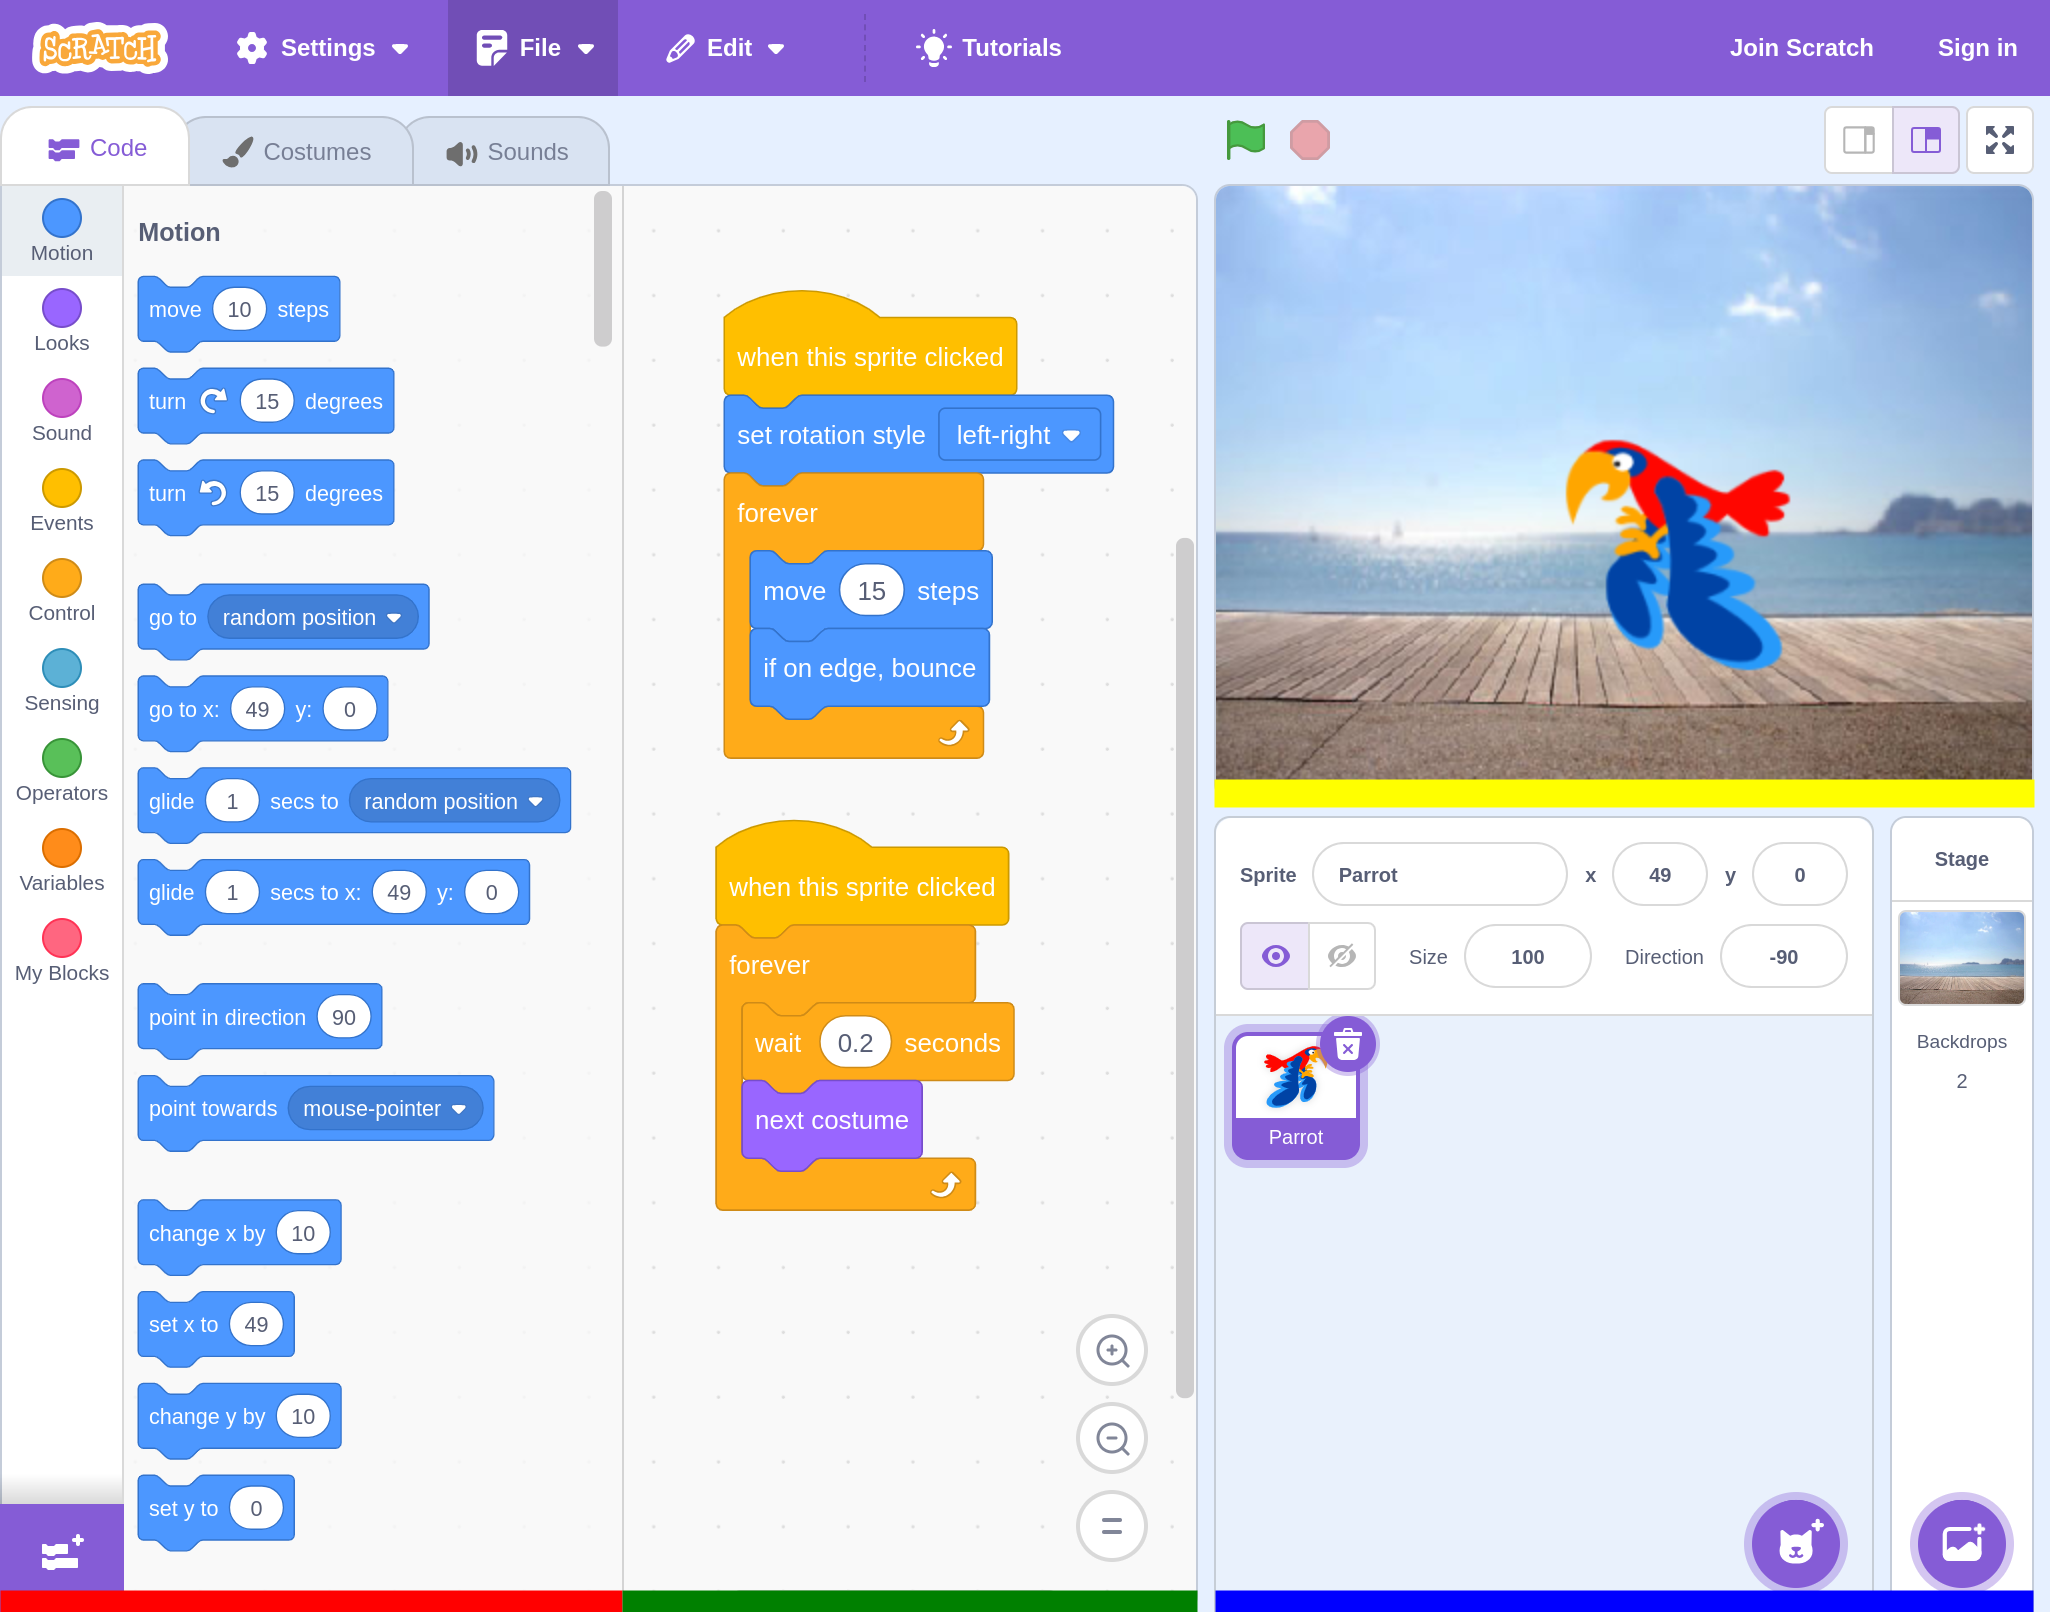
\includegraphics[width=\linewidth]{scratch-blink/scratch-normal-ide}
    \end{wide}
    \caption{The Scratch environment running an example project.
    The toolbox with the available blocks is underlined in red, the workspace is underlined in green, the editors for the sprites and the stage are underlined in blue, and the canvas is underlined in yellow.}
    \label{fig:scratch-ide-intro}
\end{figure}


\section{Internal workings and organization of Scratch}\label{sec:scratch-internal}

Scratch consists of a set of independent source code modules that work together to form the complete Scratch experience.
Below is an overview of the different modules (their relationship is shown in TODO).
In 2019, Scratch 3.0 was released.
This version is a complete rewrite to use web technologies, such as JavaScript, HTML, and CSS.
Scratch now runs in the browser.

\begin{description}
    \item[Scratch Blocks\footnote{\url{https://github.com/scratchfoundation/scratch-blocks}}] A fork of Google's Blockly, a library for building block-based computing interfaces.
    \item[Scratch Virtual Machine\footnote{\url{https://github.com/scratchfoundation/scratch-vm}}] The engine behind Scratch and responsible for running the programs created by the blocks.
    \item[Scratch User Interface\footnote{\url{https://github.com/scratchfoundation/scratch-gui}}] A React-based web application that consists of the Scratch programming environment. It uses and builds on the other components.
    \item[Scratch Renderer\footnote{\url{https://github.com/scratchfoundation/scratch-render}}] A WebGL-based renderer, responsible for rendering the canvas.
    \item[Scratch Paint Editor\footnote{\url{https://github.com/scratchfoundation/scratch-paint}}] The component that provides the editing functionality for the costumes of sprites.
    \item[Scratch Storage\footnote{\url{https://github.com/scratchfoundation/scratch-storage}}] Library for loading Scratch projects.
\end{description}

This part of the thesis deals with Scratch, an educational software testing framework.
One of its defining features is the ability to create programming-language-agnostic exercises.
This means that the same exercise (with one test suite) can be solved in multiple programming languages, without loosing automated assessment.

%\marginnote{TESTed was first started in my master's thesis.}
TESTed has produced two publications:

\begin{itemize}
    \item \fullcite{strijbolTESTedEducationalTesting2023}
    \item TODO
\end{itemize}

%The first paper is the answer to the research question: ``Is it possible to create an educational software testing framework for programming-language-agnostic exercises?''.
%The answer is yes.
%\Cref{ch:tested1} is based on that article.
%\marginnote{This thesis doesn't have a page limit, after all.}
%It has been expanded with more information about the inner workings of TESTed, in addition to going more in-depth on technical aspects of the framework.
%
%With a working prototype, we then took a step back to look at what is required to go from the prototype to a viable option for creating programming exercises.
%We want TESTed to be suitable for both educators in higher education and secondary education.
%Our ambition was to make TESTed the default options for creating programming exercises in Dodona~\autocite{vanpetegemDodonaLearnCode2023}, our platform for programming exercises.
%
%This resulted in the second paper (\cref{ch:tested-dsl}).
%We looked at software testing more broadly, and we conclude that an important part is an ergonomic and approachable way to author test suites for exercises.
%The result of this is TESTed-DSL, a domain-specific language for authoring programming-language-agnostic exercises with support for automated assessment.
%We also provide a solution to language-agnostic task descriptions.
%
%One consequence of this approach is that there is some overlap in both chapters: for example, the introductions in both chapters broadly cover the same topic.
%However, the focus in both is different enough that we feel there is no problem including both: they are not verbatim copies.
%Another example is the terminology used for the levels in the test suites (\vref{subsec:structure-of-a-test-suite} and \vref{subsec:dsl-test-suite-structure}), which have different names.
%The first chapter uses the terminology as used by Dodona, while the second chapter changes those in the DSL to align more with the terminology used in the literature.
%
%
%As a software project, the source code for TESTed is important.
%It is published\footnote{\url{https://github.com/dodona-edu/universal-judge}} under the \textsc{mit} licence, which is the tradition at Team Dodona (of which TESTed is a part).
%
%Two ``types'' of documentation are also available:
%
%\begin{itemize}
%    \item The guides for educators wanting to create programming exercises\footnote{\url{https://docs.dodona.be/en/guides/exercises/}}.
%          Most of these guides are currently only available in Dutch.
%    \item The reference documentation, for a more in-depth look or more technical subjects\footnote{\url{https://docs.dodona.be/en/references/tested/}}.
%          For example, this includes the documentation on how to extend TESTed to add support for more programming languages.
%\end{itemize}

Too often, researchers and educators are adopting automated assessment tools that evaluate student programming projects only by analyzing the code, without considering the project goals, content, design, interface, usability, or documentation. For example, many are using an online Scratch assessment tool that gives students a “computational thinking score” based on the assumption that code with more types of programming blocks is an indication of more advanced computational thinking. This form of assessment doesn’t take into consideration what the student’s program is intended to do, how well it accomplishes the student’s goals, whether the code works as intended, whether people are able to interact with it, or how the student’s thinking develops over a series of projects. We see greater potential in other research and evaluation approaches, such as those that document and analyze teachers’ facilitation practices and students’ learning trajectories over time.6,8
% https://cacm.acm.org/research/coding-at-a-crossroads/

\end{document}
